\documentclass[12pt,a4paper]{report}
%\documentclass[12pt,twoside]{report}

\usepackage{amsmath}
\usepackage{epsfig,amsthm}
\usepackage{amssymb}
\usepackage{listings}
\usepackage{hyperref}
%\usepackage{epsfig,amstex,amsthm}

\linespread{1.6}
%\linespread{2}
%\renewcommand{\baselinestretch}{2}

%\setlength{\baselineskip}{20pt}
\setlength{\topmargin}{-0.5cm}
%\setlength{\topmargin}{0cm}
\setlength{\textheight}{23.5cm}
\setlength{\oddsidemargin}{1.5cm}
\setlength{\evensidemargin}{0cm}
\setlength{\textwidth}{14.4cm}
\setlength{\headsep}{0in}
\setlength{\parskip}{.15in}
%\setlength{\parindent}{.5in}
\setlength{\parindent}{0in}

\begin{document}

\pagenumbering{roman}

\addcontentsline{toc}{chapter}{Title Page}
\null\vspace{0.5in}
%\vspace{0.5in}
\begin{center}
{\Large\bf Design and Implementation of Parallel Simulation Ranking and Selection Procedures}
\vspace{2.5cm}

{\large by}
\vspace{0.5cm}

{\large\bf WU Yang}\normalsize
\vspace{1cm}

A Thesis Submitted to \\
The Hong Kong University of Science and Technology \\
in Partial Fulfilment of the Requirements for \\
the Degree of Master of Philosophy \\
in Industrial Engineering and Logistics Management
\vspace{1.5cm}

July 2013, Hong Kong
\end{center}
\thispagestyle{empty}
\newpage

\addcontentsline{toc}{chapter}{Authorization Page}
\begin{center}{\Large\bf Authorization}\normalsize
\end{center}
\vspace{0.5cm}

I hereby declare that I am the sole author of the thesis.

\vspace{0.5cm}

I authorize the University of Science and Technology to lend this thesis
to other institutions or individuals for the purpose of scholarly research.

\vspace{0.5cm}

I further authorize the University of Science and Technology to
reproduce the thesis by photocopying or by other means, in total or in
part, at the request of other institutions or individuals for the
purpose of scholarly research.

\vspace{1.5cm}

\begin{center}
\line(1,0){180}
\smallskip

WU Yang \\
5, July 2013
\end{center}

\newpage

\addcontentsline{toc}{chapter}{Signature Page}
\null\vspace{1.0cm}
\begin{center}
{\Large\bf Design and Implementation of Parallel Simulation Ranking and Selection Procedures}
\vspace{1.5cm}

{\large by}\smallskip

{\large\bf WU Yang}\normalsize

\vspace{1cm}

This is to certify that I have examined the above MPhil thesis \\
and have found that it is complete and satisfactory in all respects, \\
and that any and all revisions required by \\
the thesis examination committee have been made.

\vspace{2.0cm}

\line(1,0){180} \smallskip

Prof. L. Jeff HONG, Supervisor
\vspace{1.5cm}

\line(1,0){180} \smallskip

Prof. Fugee TSUNG, Head of Department
\medskip

Department of Industrial Engineering and Logistics Management\medskip

5 July 2013
\end{center}

\newpage

\addcontentsline{toc}{chapter}{Acknowledgements}
\begin{center}{\Large\bf Acknowledgements}\normalsize
\end{center}
\vspace{0.5cm}

First of all, I would like to thank Prof. L. Jeff HONG, my advisor during my MPhil study. He has impacted me by showing the following facts through his words and deeds. Firstly, research could be so interesting. Secondly, a successful researcher, like him, could enjoy an academic life so much. Thirdly and most importantly, people with properties of successful researchers, like him, could have a much deeper understanding of the world we're living in.

After that, I would like to thank Dr. J. LUO, a senior lab-mate of mine. He led me to office from Choi Hung MTR station the first time I came to UST. He also led this research and got paper published on Operation Research.

Then, I would like to thank our department for supporting me with the studentship and an academic atmosphere here.

Finally, I would like to give my best wishes to all the people I meet here. Thank you for sharing this period of life with me.

\newpage
\addcontentsline{toc}{chapter}{Table of Contents}
\tableofcontents
\listoffigures
\listoftables

\newpage
\addcontentsline{toc}{chapter}{Abstract}
\begin{center}
{\Large\bf Design and Implementation of Parallel Simulation Ranking and Selection Procedures}
\vspace{0.5cm}

{\large \bf by WU Yang}\normalsize

\medskip

Department of Industrial Engineering and Logistics Management \\
The Hong Kong University of Science and Technology

\end{center}
\vspace{1.5cm}
\centerline{{\bf \large Abstract}}
\vspace{1.5cm}

Conventional simulation ranking-and-selection(R\&S) procedures are designed and implemented in serial computing environment. However, it is the trend that the growth of computing power relies more on parallelism rather than faster serial execution. The consequence is that it becomes more and more difficult for those serial simulation R\&S procedures to take advantage of the development of computing technology. In this thesis, we propose our design and implementation of simulation R\&S procedures in parallel computing environment with master-slave structure in higher level. Extensive numerical experiments show that our parallel simulation R\&S procedures is capable of large-scale problems with scalability against the number of available parallel computing units.

\newpage
\pagenumbering{arabic}

\chapter{Introduction}

The problem of selecting the best is to decide the best one within a finite number of alternatives, where the best is defined as the largest or smallest mean, which is inferred from statistical sampling, by real experiments or computer simulations. To solve such kind of problem, the ranking-and-selection(R\&S) procedures are widely adopted. In this thesis, we only focus on the case where the statistical sampling is archived through computer simulations. Consequently, the obtained simulation results are called samples, and the corresponding R\&S procedures are specifically simulation R\&S procedures.

Not very long ago when serial computing still dominants, simulation R\&S procedures are designed and implemented serially, where the most important performance issue lies on the algorithm complexity, roughly the proportion of the run-time over the problem size. Once the algorithm complexity of the procedure is settled, the time cost will decrease as the serial execution speed increases, without specifically modifying the procedure itself, even the corresponding programming implementation. In this way, a simulation R\&S procedure can easily enjoy the growth of computing power, which relies on faster serial execution speed, as long as the algorithm complexity is satisfying.

However, as we have already entered the age of parallel computing, the computing environment has significantly changed. Due to some physical limitations, the growth of computing power relies more on parallelism, rather than faster serial execution. In another word, the serial execution speed is not growing as fast as it used to be. If those serial simulation R\&S procedures still remain the same, they can hardly utilize the recent development of computing technology.

On the other hand, the demand raised from the practical applications of simulation R\&S procedures also requires us to enhance existing procedures. As is pointed out by \cite{ehiorams06ras}, the size of the problem that conventional serial simulation R\&S procedures can handle is rather small, about 500 alternatives at most. It's definitely not enough for many practical scenarios where the number of alternatives is thousands even tens of thousands. 

Traditionally, the conflicts between large-scaled problems and limited capacity of simulation R\&S procedures are solved within serial computing environment by optimization via simulation(OvS) algorithms. A recent review can be found in \cite{potwsc09ovs}. Many OvS algorithms guarantee the global convergence, namely deciding the best after spending enough simulation effort. However in most cases there won't be sufficient computing budget for enough simulation effort and those OvS algorithms will stop much earlier than then ideal point, causing the selected alternative losing statistical validity. In other words, serial OvS algorithms will eventually trade statistical validity for computational practicability, which makes it not a perfect replacement for serial simulation R\&S procedures.

On the contrary, within parallel computing environment, the computational tasks are executed simultaneously. A large problem can be divided into smaller ones, and such small problems can be carried out at the same time, thus speeding up the whole process. In typical R\&S scenarios, all the simulation efforts are naturally suitable for divide-and-conquer, and so as for parallel computing.

All the above statement motivates us to re-design and implement simulation R\&S procedures in parallel computing environment, in order to take advantage of recent development of computing technology and gain extra speed-up compared with serial R\&S. At the same time it will also dramatically enlarge the size of the problems that are suitable for applying simulation R\&S procedures, while avoid the statistical validity loss compared with adopting serial OvS.

An important issue worth being noticed here is the scalability of simulation R\&S procedures in parallel computing environment. Scalability refers to the ability of a system to increase its total capability when more resources are added. In our case, it roughly means how much better our simulation R\&S procedures perform when more parallel computing units are provided. Just like the algorithm complexity is adopted to compare serial algorithms, according their growths of running time against the increasing of problem size, thus avoiding the unfairness brought by different hardware configurations, we use the scalability to compare simulation R\&S procedures in parallel computing environment.

With the consideration of scalability, migrating serial simulation R\&S procedures into parallel computing environment becomes challenging. As is pointed out by the Amdahl's Law raised in \cite{amdahl}, once the total workload is fixed, the minimal time cost has a lower bound, which limited by the proportion of the workload which has to be carried out in serial. In general R\&S scenarios, all the workload except from pure repeated simulations are not that easy to get paralleled, which means these workload probably have to be done in serial and may become the bottle neck for the whole simulation R\&S procedure.

Except from the consideration from scalability, other tricky statistical issues also arise. In parallel computing environment, an earlier started task may finish later, since other tasks are also executing simultaneously. Specifically in R\&S scenario, the order of the starting of a sequence of simulation experiments may differ from that of the finishing of the same sequence of simulation experiments. What is worse, the latter order may be totally random. This violates some fundamental assumptions in previous simulation R\&S procedures. More discussions can be found in \cite{ras-seq-parallel}, where two new fully sequential simulation R\&S procedures, vector-filling procedure and asymptotic parallel sequential procedure, are proposed to address these statistical problems.

In this thesis we design and implement a general platform for parallel simulation R\&S procedures, with three specific procedures: Rinott's procedure (see \cite{cistam1978rinott}), vector-filling procedure(see \cite{ras-seq-parallel}), asymptotic parallel sequential procedure (see \cite{ras-seq-parallel}), and two specific simulation experiments: $(s, S)$ inventory simulation(see \cite{cissac1985ss}), three stage buffer allocation simulation(see \cite{smoms93threestage}). At any active time, the whole platform consists of three major components, of which the most essential one is a general framework. This framework contains the fundamental work for the parallelism of simulation R\&S procedures, with master-slave architecture in high level, which is a pretty common pattern in software design. The other two are specific procedure and specific simulation experiment, respectively. These two components are implemented as plug-ins of the whole system, no matter the three procedures and two simulation experiments already implemented by us, or any possible procedures and simulation experiments implemented by anyone in the future. In this way, extensibility is archived. Meanwhile, the most important goal we have archived is its high scalability proved in numerical experiments.

Our work is related to three streams.

The remainder of this thesis is organized as follows. Chapter 2 covers the related background information, including recent development of simulation R\&S procedures and basic theories and technologies of parallel computing. We describe our work in a top-down manner in chapter 3, with parallelism of each simulation R\&S procedures analysed and extensive numerical results presented. Comparison acceleration in serial part of R\&S is discussed in chapter 4, followed by conclusions and some future work in chapter 5.

\chapter{Background}

\section{Simulation R\&S Procedure}

\subsection{Problem of Selecting the Best}

The problem of selecting the best is common in operation research. Here we give two examples, related to safety stock and efficient manufacturing, respectively. Both of them can be carried out by discrete event simulation experiments.

\subsubsection{$(s, S)$ Inventory Model}

This is about setting up reordering point in inventory management and it once appeared in \cite{cissac1985ss}. A general model with two parameters $s$ and $S$ works in the way that as long as the inventory level goes below $s$, then an order with the amount $S - s$ will be send out, after which the inventory level will regain to $S$. This is the $(s, S)$ inventory model. And in order to apply this model, extra effort is needed to specify $s$ and $S$ in each practical case to minimize the reordering cost.

In this example, both $s$ and $S$ are limited in specific problem instances, like $S$ must be less than the capacity of inventory store, $s$ must between $0$ and $S$, both $s$ and $S$ must be natural numbers, which is often the case. Consequently the number of feasible combinations of $s$ and $S$ are limited in finite. The performance we're interested here is the reordering cost, so the best combination of $s$ and $S$ is defined as the one with the smallest expectation of the reordering cost. In this way, a practical inventory management problem can be treated as the problem of selecting the best.

\subsubsection{Three-stage Buffer Allocation}

This is about allocating buffer space in a multi-stage manufacturing line and it once appeared in \cite{smoms93threestage}. Let's take a three stage manufacturing line as an instance. In this case, there are three manufacturing units, or stages, in a manufacturing line, and each stage has its own capacity for manufacturing items. In front of the second stage and third stage, there exist a buffer space, respectively. which also has its own capacity for manufacturing items. In this model, there're five parameters representing capacities in five locations including the three manufacturing units and two buffers. The manufacturing manager needs to specify these five parameters to archive maximum throughput for the whole manufacturing line.

Just the same as the previous example, the total number of manufacturing items inside this manufacturing line, or the summation of these five parameters, is limited in specific problem instances. What's more, these parameters also need to be natural numbers in most cases, thus limiting the number of feasible combinations of these five parameters into finite again. What we're interested in here is the throughput of the whole manufacturing line and the best combination of these five parameters is defined as the one which makes the largest expectation of throughput. Again in this way, the practical three-stage or multi-stage buffer allocation problem can be treated as problem of selecting the best.

\subsection{R\&S Procedures}

During the past, many R\&S procedures have been developed to solve the problem of selecting the best, with literature view papers like \cite{ras-recent-advances}, \cite{ehiorams06ras} and \cite{ms05ras}. Typically, they allocate simulation effort to all alternatives, namely, running simulation experiments repeatedly for a specified finite number of times against all the alternatives. Here each alternative is distinguished by a vector of arguments. The goal is to guarantee certain statistical validity when making selection decision, such as the probability of correct selection, or PCS for short.

Although many other types of R\&S procedures exist, in this thesis only several representative ones get involved to illustrate our idea. We only take a frequentist’s view and consider the formulation of indifference-zone, or IZ for short. IZ is proposed in \cite{toams1954iz} and recent summary can be found in \cite{nyjws95iz}. We will briefly review two classic R\&S procedures later.

\subsubsection{Rinott's Procedure}

Rinott's procedure is a classic R\&S procedure developed in 1978 by Rinott in \cite{cistam1978rinott}. It guarantees with the confidence level $1 - \alpha$ that the alternative get selected is at least $\delta$ better than the second best one. If alternatives within $\delta$ worse than the best one exist, then Rinott's procedure guarantees to select one of these "good enough" alternatives with the same probability. The $\delta$ here is called indifference-zone. It is set by procedure user to determine the smallest difference that is worth getting noticed. In other word, differences less than this $\delta$ can be ignored from a practical viewpoint.

Suppose there are $k$ systems where $k \geqslant 2$. Let $X_{ij}$ denote the $j$th independent sample value from simulation experiments of alternative $i$. We assume that $X_{ij} \backsim N(\mu_i, \theta_i^2)$, where both $\mu_i$ and $\theta_i^2$ are unknown, and each $X_{ij}$ is independent from each other. Also let $\bar{X_i}(r) = r^{-1}\sum_{j=1}^r$, namely the sample mean of first $r$ sample values of alternative $i$, and let $S_i^2 = \frac{1}{n_0 - 1}\sum_{j=1}{n_0}(X_{ij} - \bar{X_i}(n_0))^2$, the sample variance of first $r$ sample values of alternative $i$.

With these symbols, we organize the Rinott's procedure as following steps:

\begin{enumerate}
\item{Set up: } Set up parameters $\alpha$, $\delta$ and $n_0$. $n_0$ is the sample size in first stage and $n_0 \geqslant 2$.
\item{Initialize: } Calculate Rinott's constant $h = h(n_0, k, 1 - \alpha)$ with method mentioned in \cite{rinott-constant}. Collect $n_0$ independent sample values $X_{ij}$, where $j = 1, 2,...,n_0$, for each alternative $i$, by repeatedly running simulation experiments against that alternative, and for $i = 1, 2,...,k$, calculate $S_i^2$. Let 
$$ N_i = \max\{n_0, \lceil \frac{h^2S_i^2}{\delta^2} \rceil\} $$ where $N_i$ is the number of sample value that will eventually taken from alternative $i$.
\item{Stopping Rule: } If $n_0 \geqslant \max N_i$ then stop and select the alternative with the best sample mean, namely the largest or smallest $\bar{X_i(n_0)}$. Else take $\max\{N_i - n_0, 0\}$ extra sample values from each alternative $i$ by continue repeating the simulation experiments, after which select the alternative with largest or smallest $\bar{X_i(N_i)}$ as the best.
\end{enumerate}

And specifically, if the best alternative is defined as the one with largest expectation, then Rinott's procedure guarantees
$$ Pr\{\text{select alternative i }|\text{ }\mu_i - \mu_j \geqslant \delta \} \geqslant 1 - \alpha $$
where $1/k < 1 - \alpha < 1$. Since this thesis focuses on implementation, reader interested in the proof may refer to \cite{ras-recent-advances}. 

One related issue worth mentioning here is that the total sample size required in Rinott's procedure is slightly less that $O(k\log{k})$, which determines the total computing effort.

\subsubsection{A Fully Sequential Procedure}

While the Rinott's procedure mentioned above is a classic two-staged procedure, fully sequential is another important type of procedures, with classic examples like KN in \cite{tomacs01kn} and NSGS in \cite{or01nsgs}. However the procedure we will review right after this paragraph is a newly developed one also featured as fully sequential. It first appears in \cite{ras-seq-jeff} by L. J HONG in 2004. This procedure provides good statistical validity while keeps a great opportunity of decreasing total number of sample values, approximately the total computing effort need to spend, at same time. The key point is that if at any time there is enough evidence to prove that some certain alternative is clearly inferior, then this alternative will get eliminated immediately in theoretic like what most fully sequential procedures do.

With the symbols same as those in Rinott's procedure, we organize the this procedure as following steps:

\begin{enumerate}
\item{Set up: } Set up parameters $\alpha$, $\delta$ and $n_0$. Let $\lambda = \eta / 2$ and $a$ be the solution of the equation below:
$$ E[\frac{1}{2}\exp(- \frac{a\delta}{n_0 - 1} \Psi)] = 1 - (1 - \alpha)^{\frac{1}{k - 1}} $$,
where $\Psi$ is a random variable with PDF
$$ f_{\Psi}(x) = 2 [1 - F_{\chi_{n_0 - 1}^2}(x)] f_{\chi_{n_0 - 1}}^2(x) $$,
and $F_{\chi_{n_0 - 1}^2}(x)$ and $f_{\chi_{n_0 - 1}}^2(x)$ are the CDF and PDF of $\chi^2$ distribution with $n_0 - 1$ degrees of freedom.
\item{Initialize: } Let $I = {1, 2,...,k}$ be the set of current surviving alternatives. Again collect $n_0$ independent sample values $X_{ij}$ where $j = 1, 2,...,n_0$ and $i = 1, 2,...,k$ by repeating simulation experiments against corresponding alternatives. Let $r$ be the counter of total number of samples and $n_i(r)$ be the number of samples of alternative $i$. Till now, $r = kn_0$, and $n_1(r) = n_2(r) = ... = n_k(r) = n_0$.
\item{Screening: } For all $i,j \in I$ and $i \neq j$, let 
$$ \tau_{ij}(r) = [\frac{S_i^2}{n_i(r)} + \frac{S_j^2}{n_j(r)}]^{-1} $$
and
$$ Y_{ij}(\tau_{ij}(r)) = \tau_{ij}(r)[\bar{X_i}(n_i(r)) - \bar{X_j}(n_j(r))] $$.
Let $I^{old} = I$, then
$$ I = I^{old}/\{i \in I^{old}: \exists j \in I^{old} \text{s.t. } Y_{ij}(\tau_{ij}(r)) < \min[0, - a + \lambda \tau_{ij}(r)]  \text{and } j \neq i\} $$
\item{Stopping Rule: } If $|I| = 1$ then stop and select the only alternative in $I$ as the best. Else let $r = r + 1$, take the $r$th sample by running simulation experiment, update $n_i(r)$ for all $i \in I$, and goto \textbf{Screening}.
\end{enumerate}

A missing specification of the above procedure lays in the part of stopping rule, namely the decision of which alternative is the next sample value from, or in other words, which configuration should be used in next replication of simulation experiment. This decision making rule is called sampling rule.

In \cite{ras-seq-jeff}, such sampling rule is applied: after first stage, run next simulation experiment against the surviving alternative with the lowest $n_i(r)/Si$. If a tie exists, run next simulation against the surviving alternative with lowest $S_i$ among them.

The sample size of such fully sequential procedures is typically smaller than that in Ronott's procedure except for some extreme case. Interested reader may refer to \cite{ras-seq-jeff} for detailed properties as well statistical validity proofs.

\section{Parallel Computing}

\subsection{Different Parallelism Levels}

In terms of granularity, parallel computing can be divided into three different levels: bit level, instruction level and task level.

\subsubsection{Bit-Level Parallelism}

Bit-level parallelism is related to the size of computer word. Inside the processor, several bits are manipulated together, which composes a computer word, and the size of computer word is defined as the number of bits it contains. More hardware details can be found in \cite{pca97} Historically, 4-bit computer word has been replaced by 8-bit, then 16-bit, 32-bit, until today's 64-bit. Although not very close to ordinary people, computer with 128-bit computer word or even larger one has been made.

\subsubsection{Instruction-Level Parallelism}

Instruction-level parallelism is a more interesting topic in computer architecture. An instruction is a computer word with special meaning for processors. Any computer program will essentially become a stream of instructions before getting executed, no matter what programming language it is written in. These instructions will get re-ordered and grouped before executing, certainly without changing the result of original instruction stream. Besides, an instruction can be divided into several stages, with each stage corresponding to a certain action, such as instruction fetch, decode, execute, memory access, write back and so on, which enables the instruction pipeline in modern processors. In addition to pipeline, the pipeline units inside some modern processors can even handle more than one action at a time, which is known as super-scalar.

Before instruction-level parallelism is adopted, the instructions inside a stream are executed serially. At any time, there is at most one instruction getting executed. The next instruction won't start unless the previous one finishes. Under such circumstances, the execution time is easy to calculate, which equals the average execution time per instruction, multiplied by the number of instructions. Without changing the amount of instructions inside a stream, the only way to decrease the execution time is to increase CPU clock frequency, which is called frequency scaling.

However, frequency scaling is limited by many physical constraints, like power consumption, heat generation and so on. Thus instruction-level parallelism has become a way out under current physical constraints, and attracts many researchers in the field of computer architecture.

\subsubsection{Task-Level Parallelism}
\label{sec:pseudo-multi-tasking}

Task-level parallelism is a higher level parallelism in the sense that it needs support from both hardware and software. In another word, both bit-level parallelism and instruction-level parallelism are implemented inside processors, making them transparent, or invisible to software. Even operating system, the most fundamental software inside computer, do not have control on bit-level and instruction-level parallelism. 

Earlier computers without task-level parallelism can also support multi-tasking, since multi-tasking operating system takes care of switching different tasks back and force from time to time according to some strategy, including saving and restoring context for each task, and does not have to wait until current task finishes. From the viewpoint of a user, the computer is doing task in parallel, but precisely speaking, such fake parallelism should be called concurrency. 

As for modern computers with task-level parallelism support, like multi-core or multi-processor, which will be introduced later, they do have the ability to make different tasks executing in real parallel, certainly also with the support from software. We will look into the details of how hardware and software support parallel in the next two sections.

\subsection{Hardware Parallel Support}

\subsubsection{Multi-core Processor}

Computers with Von Neumann architecture, which is still the dominant computer architecture today, will have at least one processor inside. For a processor, it can contain more than one execution units, or cores, on the same chip. Such processor is known as multi-core processor. Different cores inside the same multi-core processor can handle different instruction streams at the same time, thus achieve the real parallel. By the way, a core can also be super-scalar, thus handles multiple instructions from the same instruction stream. As for Intel's Hyper-Threading technology, which uses the same core to handle a different instruction stream when this core get into idle for some reason, is a form of pseudo multi-core processing.

\subsubsection{Multi-processor Computer}

One step further from multi-core processor, a computer can have more than one processors, like SMP, standing for symmetric multi-processor, which is a single computer equipped with multiple identical processors. The existence of multiple processors inside the same computer brings about the issue of accessing memory and communicating with each other.

A computer where every address of memory can be accessed within equal latency and bandwidth is recognized as Uniform Memory Access(UMA), otherwise it belongs to Non-Uniform Memory Access (NUMA). SMP is one kind of Uniform Memory Access, while MPP, standing for massively parallel processor, which is a single computer with multiple networked processors, belongs to Non-Uniform Memory Access.

Communication among processors of the same computer can be implemented in many ways, from a simple shared media like memory or bus to complicated internal network involving topologies like star or ring and routing strategies if some processors are not connected directly.

\subsubsection{Cluster}

A group of standalone computers can be connected via network to compose a cluster. Since these connected computers work together, this cluster can be regarded as one powerful computer. A cluster composed by multiple identical computers connected via TCP/IP Ethernet local area network is called Beowulf cluster, which is the most common type of cluster.

Computers composing a cluster does not have to be identical with each other, which can increase the flexibility, but also increase the difficulty for load balancing. Except from the extra network compared to single computer, other technical issues like configuration, monitoring even fault tolerance also create challenges that can't be ignored.

\subsubsection{Distributed Computing}

In a narrow sense, distributed computing means using computers communicating over the Internet to work together on a certain problem. Comparing with a cluster, communication cost over the Internet is much higher since the throughput is low while the latency may be unstable. So typically such distributed computing only deals with embarrassingly parallel problems in which communications among sub-problems are not that frequent. SETI@home is one of the best-known example of such distributed computing.

In a wider sense, distributed computing means multiple computational entities, or nodes, with their own local memory and communicating by message passing, working together to archive a certain goal. If these nodes are deployed on different physical machines in a cluster, they possess their own local physical memory and pass messages through network protocols. On the contrary, if they're deployed on the same physical machine, then the nodes are degenerated to local processes and possess their own virtual memory only. Processes on the same physical machine can certainly pass messages through network protocols via local loop network as if they're on different physical machines, but they can also choose to communicate through local operating system as a more efficient choice. For the concept of process, we will introduce it in the next paragraph.

\subsection{Software Parallel Support}

\subsubsection{Process upon Operating System}

Process is a fundamental concept in operating system. In \ref{sec:pseudo-multi-tasking}, we introduced how multi-tasking operating system make multiple tasks executed concurrently without hardware task-level parallelism. Here, the tasks should be called processes. Even with the hardware task-level parallelism, modern operating systems also regard different tasks as different processes, and provide basic services like scheduling execution on multiple cores or processors, pass messages if processes need communication, thus taking advantage of the real parallelism ability from corresponding hardware.

Formally speaking, process is an executing instance of a computer program. A computer program alone contains only static instructions, while a process also contains current execution status. Off course, multiple processes can be different instances from the same program.

With the help of operating system, processes are isolated from each other, in the sense that processes have no idea whether they're sharing CPU, memory or other computing resources with other processes, as if they occupy the whole computer, although actually the CPU is time division multiplexed while memory is space division multiplexed. Nevertheless, in this way programmers can focus on one program without considering other processes on the same machine.

On the other hand, processes on the same physical machine can communicate with each other through mechanisms provided by operating system, like shared memory, pipeline, where the output of one process get passed to another as input, and so on.

Achieving parallelism through multiple processes is based on the underlay distributed memory architecture, even they're on the same physical machine, since the operating system isolated the memories by virtual memory mechanise. Another famous memory architecture is called shared memory architecture, and we will use the concept of thread to illustrate it in the next paragraph.

\subsubsection{Thread inside Process}

Thread is a lighter concept compared with process in the sense that it is always contained inside a process. A process can have multiple threads, but at least have one, the "main" thread. Scheduling and cooperating multiple threads inside the same process involves less about operating system, thus saving computing resources. Besides, the underlay shared memory architecture, covering the memory spaces of containing process, has also provided more convenience and flexibility for programmers.

Except from thread, or precisely the POSIX Thread, OpenMP is another most widely used shared memory API. API is short for Application Programming Interfaces and can be regarded as the conventional way to use libraries installed on or provided by operating system. Both two APIs are supposed to be provided on different operating systems, in another word, cross-platform. However, the API related to process will be different if they're on different kind of operating systems since its highly coupled with underlay operating system and not cross-platform.

\subsubsection{Communication through Protocol}

The only way for processes deployed on different physical machines to communicate is via network, thus network communication protocols are involved. In other words, network protocols are involved within distributed computing. Network protocol is a set of rules for exchanging messages among computers. No matter whether communicating computers are identical or not, they can communicate with each other as long as they use the same network communication protocol.

Network communication protocol is layered. The theoretical standard is OSI model with seven layers, while the practical standard is TCP/IP model, which only has for broad layers: link layer, Internet layer, transport layer and application layer.

For software developers of distributed application, including pure parallel computing, the design decision starts varying from the Transport layer, with basically two big choices: Transmission Control Protocol(TCP) or User Datagram Protocol(UDP). TCP provides reliable, ordered, error-checked delivery of data, while UDP is connectionless and emphasizes more on lowered overhead and reduced latency. In other words, using UDP brings the chance to speed up communication with the risk of possible invalid transmitted data. Software developers of distributed application can choose to ignore the risk or pay more code on ensuring transmitted data.

Beyond transport layer, software developers also need to make design decision of application layer, say, to use existing protocols like HTTP or develop application specified protocol. HTTP stands for Hypertext Transfer Protocol and is based on client/server model. It is well supported in most dominant programming languages in format of library thus quite easy to use. Developing application specified protocol based on TCP or UDP may gain extra performance but also cost more effect and taking the risk of non-robustness.

\subsection{Performance and Scalability}

\subsubsection{Speed-up Ratio}

Speed-up ratio shows how much a parallel program is faster than its corresponding sequential program. It's defined in the following formula:

$$ S_n = \frac{T_1}{T_n} $$

Here $n$ is the number of parallel execution units, $T_1$ is the execution time of the sequential program and $T_2$ is the execution time of the parallel program with n parallel execution units. Linear speed-up or ideal speed-up is archived when $S_n = n$. 

We also defined efficiency as

$$ E_n = \frac{S_n}{n} = \frac{T_1}{nT_n} $$.

It's typically between zero and one, estimating how well the computing power is utilized, or how much cost is brought by communication or other issues. A trivial case is linear speed-up parallel program will always have an efficiency of 1.

\subsubsection{Amdahl's Law and Gustafson's Law}

Linear speed-up is only an optimally case. Most parallel programs will have a part of the program which is serial, or can not be paralleled at all, and it is this part of serial program will eventually limit the overall speed-up available from parallelism. This is the fact pointed out by Amdahl's law, which defines the speed-up ratio as:

$$ S_n = \frac{1}{(1 - p) + \frac{p}{n}} $$

Here $n$ is the number of parallel execution units, $p$ is the portion of program that can be paralleled, thus $(1-p)$ is the portion of the serial part. As $n$ goes to infinity, we have:

$$ \lim_{n \to +\infty} S_n = \lim_{n \to +\infty} \frac{1}{(1 - p) + \frac{p}{n}} = \frac{1}{1 - p} $$

And this is the maximum speed-up we can archive from parallelism, no matter how well we do in other aspects like scheduling or communication, as long as the portion that can be paralleled is fixed.

Amdahl's Law is pessimistic in the sense that once the computation amount is fixed we can only archive a limited speed-up ratio. However, from another viewpoint of fixing the total execution time instead of total computation amount, we have the optimistic Gustafson's law, which defines the speed-up ratio as:

$$ S_n = (1 - p) + n \times p $$

Here $n$ and $p$ is still the same meaning as what they're in Amdahl's Law but the speed-up ratio does not have a upper limit as $n$ goes to infinity any more.

Be attention that both Amdahl's law and Gustafson's law assume that the execution time of the serial portion of the program is independent of the number of execution units, which always violated in practise.

\subsubsection{More Affecting Issues}

The first issue is the dependency, which appears when computing depends upon prior result. These computation must be carried out in order, thus forming a dependence chain and explains how serial portion in a parallel program exists. No program can run more quickly than the longest chain, which is also known as the critical path.

The second one is race condition, which appears when two or more executing units update a certain variable at the same time and causing errors. This is because the two instruction streams can cross with each other in any order. For example, if both executing units would like to read a variable a, plus it by one, then write result back, the actual execution order could be one executing unit read a's value between the other executing unit's read and write back, thus making the final result equals to a's original value plus 1 rather than 2.

The way to solve race condition is using a lock to provide mutual exclusion when accessing variables shared to multiple execution units, thus making the whole process serial, behaving in a deterministic way and guarantee the correctness. However, here the serial portion will be linear to the number of executing units, which violates the assumption of both Amdahl's law and Gustafson's law.

Barrier is a special format lock for synchronization purpose. Basically synchronization here means two or more executing units join up at a certain point, for example, before print out all the final result. Then a barrier is used to stop the instructions after the join point from executing before every executing units reach this join point.

The third issue is deadlock, appears when multiple locks are involved. For example, if executing unit one locked variable a, and tried to lock variable b, while executing unit two locked variable b, and tried to lock variable a, then both executing units will wait for each other to release the mutual exclusion of the variable it is waiting for. This situation is called deadlock and the program will never finished. Some lock-free and wait-free algorithms can avoid the usage of lock or barrier, but they're more difficult to implement and suitable use cases are limited.

There're still many other issues not mentioned here but also need to take consideration before carrying out parallel computing.

\chapter{System Construction and Evaluation}

\subsection{Scalability Issues found in Applying R\&S to Selecting the Best}

Scalability is generally hard to define. In the case of simulation R\&S, it can be defined as the ability to handle a growing number of alternatives, with proportional computing resource added.

Although existing R\&S procedures have gained great achievement in theoretical areas like statistics, practically these procedures can hardly handle scenarios where the number of alternatives is huge. As pointed out by Kim and Nelson (2006a), the two-stage Rinott’s procedure is typically applied when the number of alternatives is fewer than 20. As for fully sequential procedure KN, the number is considered as no more than 500. Other procedures like NSGS which claims to have been designed specifically to solve large-scale R\&S problems, reported 500 alternatives as the largest test case in their paper. However in practice, it is common to have thousands even tens of thousands of alternatives needed to be considered, which has exposed the shortcoming of scalability in R\&S.

\subsubsection{A Theoretical Make Up}

Traditionally, the shortcoming of scalability in R\&S are made up through solutions of optimization-via-simulation, or OvS for short. OvS is a kind of solutions, or algorithms, which also aims at the problem of selecting the best. It guarantees global convergence, namely when simulation effort goes to infinity, it can eventually guarantee the correct selection of best.

However, the infinite simulation effort means exactly the R\&S procedures. In most of the cases, OvS algorithms will stop so early at some point that it is still quite far way from infinity, which consequently breaks the statistical guarantee of optimal selection. What is worse, the result give by the OvS algorithm may be significantly inferior to the optimal one, making it useless to the selecting of the best problem. 

Essentially speaking, any OvS algorithm will sacrifice statistical guarantee for time-saving through partially applying R\&S. Therefore, it is only a make up solution with trade-off between statistical guarantee and time cost.

\subsubsection{A Possible Way Out from Implementation}

Since trading off between statistical guarantee and time cost looks like a zero-sum game, we do hope to find a way that can deal with practical-sized problem of selecting the best, with both fully applying R\&S procedures to archive statistical guarantee, and decreasing the time cost to a reasonable amount so that we can afford to wait. A possible way out is from implementation.

As is pointed out by Moore's law proposed in \cite{moore}, available computing powerful is becoming more and more sufficient, with a speed of doubling itself every 18 months. But fully taking advantage of the fast-growing computing power nowadays is not as straightforward as it used to be, since the time of serial computing, when the growth of computing power relays on serial execution speed, has already past, and we're in the age of parallel computing.

\section{Parallel Implementation of Ranking and Selection Procedure}

As can be seen from above, due to the complicated way in which the computing power grows in the age of parallel computing, it is impossible to gain speed-up in problem solving without carefully design a parallelism plan against targeted problem. There exists previous work that use parallel and distributed computing to deal with single extremely long-running simulation in \cite{potwsc05ras}, with typical examples by Fujimoto in \cite{cotacm90fuji} an \cite{scsmasm10fuji}. However in current R\&S scenario it is the huge number of repeated simulations rather than the time cost of single simulation that matters. Now we will start this part by analysing the parallelism inside the existing procedures.

\subsection{Parallelism Analysis of Existing Procedures}

Independent is a frequently appeared modifier in literatures of R\&S. Although this modifier is kept mainly for ensuring good statistical properties of sample values, it also save us much burdens redesign R\&S into parallel.

However that's only for the simulation, or sampling part. The procedure itself is completely in a serial style, namely one step is often dependent on the one prior to it. Sometimes even loops exist among steps. This serial style composes an implicit dependency chain, and becoming the potential performance bottle-neck for the whole implementation.

Now let's look into the two representative procedures we have reviewed before.

\subsubsection{Rinott's Procedure}

In the beginning part of Ronott's procedure, things like setting up the parameters and calculating the Rinott's constant have to be done serially.

Later sampling tasks in the initialize step, or first-stage, can be paralleled due to the independence. However, a hidden lock, or barrier lays here, since we have to wait until all the simulation experiments return its result, or sample value before we move on to the next step. Luckily to archive load balance here is quite easy.

As for the sampling tasks in the stopping step, or second-stage, it is similar to those mentioned above, only differs that the required sample numbers of different alternatives are not the same, which doesn't affect parallelism at all. Again, a implicit barrier is needed before we report the final selection.

Besides, the calculation after each barrier should be considered as the serial part of the whole program.

Anyway, Rinott's procedure is fairly easy getting paralleled.

\subsubsection{Fully Sequential Procedure}

Although Rinott's procedure can get paralleled with fairly little effort, there is still enough motivation for us to study the parallelism of fully sequential procedures, since such procedure can solve problem with smaller sample size, namely total computing effort in terms of serial computing. Let's still take the one in \cite{ras-seq-jeff} as an example.

In the beginning part of this procedure, it's the same as Ronott's procedure and work here has to be done serially.

In the first-stage, it's exactly the same as Ronott's procedure, say embarrassingly parallel ends with a barrier.

However in the second-stage, things become totally different and much more interesting. Basically, the original idea is to repeat the process of taking a sample value, or running a simulation experiment, against certain alternative, then do some calculation globally to see whether some alternative can get eliminated, until there's only one alternative surviving. Let's dig out the parallelism here bit by bit.

Firstly, we don't need to run simulation experiment only one at a time, why not start as many simulation experiments as we can, as long as we do have so many task-level parallel executing units?

It looks reasonable but at least the corresponding sampling rule needs to be modified to adapt to parallel environment. Besides, even after the modification of sampling rule, another problem of the reordering of the sample obtaining sequence compared to the specified sampling sequence appears. It is due to the uncertainty of which sub-task would be finished earlier even we start these sub-tasks "at the same time" and all the executing units are "identical". The double quotes here means that it is hardly controlled by us whether these sub-tasks are started exactly at the same time and whether these executing units are exactly identical. It's not a big deal and happens in almost every parallel program, but it does become a critical issue in theoretic since it challenges the original implicit assumptions based on which the essential statistical properties are maintained.

Secondly, do we have to carry out the global calculation, or more precisely the comparison, every time after we obtain a sample value?

It should be noticed that, carrying out a global comparison will need mutual exclusive protection, otherwise the appearance of a new sample value during the comparison will make global data inconsistent for this comparative calculation. In other words, a global comparison is expensive in parallel environment.

Solutions based on decreasing comparison time sounds reasonable, but they waste elimination chances in potential. Besides, existing theory does not offer enough support.

All these trouble lays on the point that the original typical fully sequential procedures are not designed specifically for parallel environment at all. It's time to revise conventional fully sequential R\&S procedure and we will introduce two revised fully sequential procedures which are more suitable in parallel environment, in the next section.

\subsection{Revised Fully Sequential Procedures}

\subsubsection{Vector Filling Procedure}

The basic idea for vector fill procedure, or VF for short, is sticking to perform comparisons based on the originally specified sampling sequence, by using an vector recording the sampling values exactly in the order specified by the sampling rule.

In this way, the first problem mentioned above get solved with the original statistical validity staying unchanged. However as for the second problem, the VF procedure may not use all obtained sample values at the time of each comparison, although procedure users do have a control on comparison opportunity.

From the viewpoint of implementation, the most critical issue is that essentially the VF procedure is to sacrifice space for statistical validity. The space here could be memory space only, with improving opportunity from self-customized memory management policy, or switching back and force from hard disks to memory if total memory space can not afford the whole vector, which will definitely slow down the computation dramatically since hard disk accessing always costs much more time than memory accessing.

\subsubsection{Asymptotic Parallel Sequential Procedure}

VF procedure is conservative in the sense that in order to keep most statistical validity it does not utilize all the obtained sample values, which loses many potential chances to eliminate inferior alternative earlier, thus is not that satisfying in speeding up the whole process.

To over come this weakness of vector filling procedure, asymptotic parallel sequential procedure, or APS for short, is developed to allow unequal sample sizes for all alternatives and make elimination decisions based on all obtained sample values. It has been shown that the asymptotically validity can be guaranteed as the indifference-zone parameter goes to zero. Interested reader may refer to \cite{ras-seq-parallel} for more details.

Since APS procedure can fully utilize all the obtained sample values, it is definitely more efficient in eliminating inferior alternatives than VF. Besides, APS procedure doesn't require recording all the sample values obtained. It only needs some summarising information of obtained sample values like summation, summation of square and so on, which can be updated as new sample value obtained. This feature lowers the storage space demand and in this way the whole data of APS procedure can be easily fit into main memory, which guarantees the order of computing speed.

\subsection{Architecture Based on Master-Slave}

With the revision of existing fully sequential R\&S procedures, now it is possible to implement serial ranking and selection within an architecture for parallel execution. We will adopt the master-slave pattern as the higher lever architecture for its flexibility to support features aside of embarrassingly parallel part in R\&S procedures and scalability to deal with the large-scale size in selecting the best problem. Besides, it is also fairly easy from a implementation viewpoint.

As is introduced in section 3.5.3, master-slave means a master execution unit dealing with the serial part while several slave execution units share the workload which can be carried out in parallel. In the current scenario, the ranking and selection, including specifying sampling rule and making elimination according to obtained sample values from simulation, should be implemented on master, while the independent simulation experiments should be shared among all the slaves, with scheduling from the master.

In this section we will mainly introduce this architecture inside the scope of a single machine, where the whole program is inside a single process and master or slaves are all threads inside this process. At the end we will take a look at scaling it out to a cluster.

\subsubsection{Master}

As is mentioned above, master will take charge of essential serial steps in ranking and selection procedures, and one thing that should be noticed here is that the master part is not exactly the main thread for the whole program, since there's more "duty" work left to do in the main or entrance thread like parsing parameters of R\&S procedure, inputting the configurations of every alternative and other program level configurations like number of slave threads or directory for log files. Interested reader should refer to the code directly.

At the end of the main thread, when everything is ready including separated slave threads, the main thread will start the execution of master part and end when the master part is done, at which point the whole program is terminated.

For the universality of this implementation, here the logic of ranking and selection procedure is called through a abstract programming interface. To make this clear, readers should first noticed that our implementation can be divided into two major parts. One part includes the core components, the other consists of implementations of different R\&S procedures and different simulation experiments. Every time user of our implementation should choose one specific implementation of R\&S procedure and one specific implementation of simulation experiments, and start this R\&S program together with all the core components.

In other words, the core components are programmed with only dependent on the abstract function signatures of both R\&S and simulation. This follows an important design rule, say, depend on abstract rather than implementation. In this way, the core component part can stay unchanged against the change of R\&S and simulation.

As for the detailed specifications of R\&S implementation and simulation implementation, we will look into details in later part specifically introducing the extension point for self-customized R\&S procedure. And till now we have finished introducing the very abstract master, which is started from almost the end of the main thread and interacts with specific ranking and selection logic through abstract programming interfaces.

\subsubsection{Slave}

Generally speaking, there should be multiple instances of slave within a master-slave structure. Within the single machine scope, a slave instance is a dedicated thread and different slave threads are identical in code while different in the data it is processing and the status it is in.

All the threads except from the main thread are started within the main thread, including the dedicated slave threads here. Advanced thread starting technique like thread pool are involved here to archive better scheduling. Interested reader may refer to the code.

Briefly speaking, there are three steps inside a working cycle of slave thread, they're simulation argument fetching, simulation experiment executing and simulation result submitting. The slave threads will follow this working cycle one round after another until explicitly stopped.

Both argument fetching step and result submitting step involve communication with the master, or ranking and selection logic, which is considered as extra cost introduced by adopting parallel computing. We have used two FIFO queues to buffer the arguments and results to reduce such communication cost. Detailed buffering policy will be illustrated in later section with the name buffered communication.

As for the simulation step, again it is done simply by calling the abstract programming interface of simulation task, thus supporting self-customized simulation experiments. Specification of this programming interface will be described in later section.

\subsubsection{User Interface}

In order to reduce the study cost of users who adopt our implementation, well designed user interface is necessary part in the whole system. In our implementation, the user interface can be divided into two kinds. One is for users using our implementation directly, the other is for users extending in ranking and selection procedure and simulation experiment.

For the first kind of user interface, we could simply leave a command line interface since it is only an academic purpose software tool. However, since at the end of day we would like it to become a computing service, or more precisely, cloud computing, which distributes computing service to end user via Internet, we developed a web interface for it, as a prototype for that stage. Here is a screenshot of that web page:

\begin{figure}[ht]\label{web-ui}
\centering
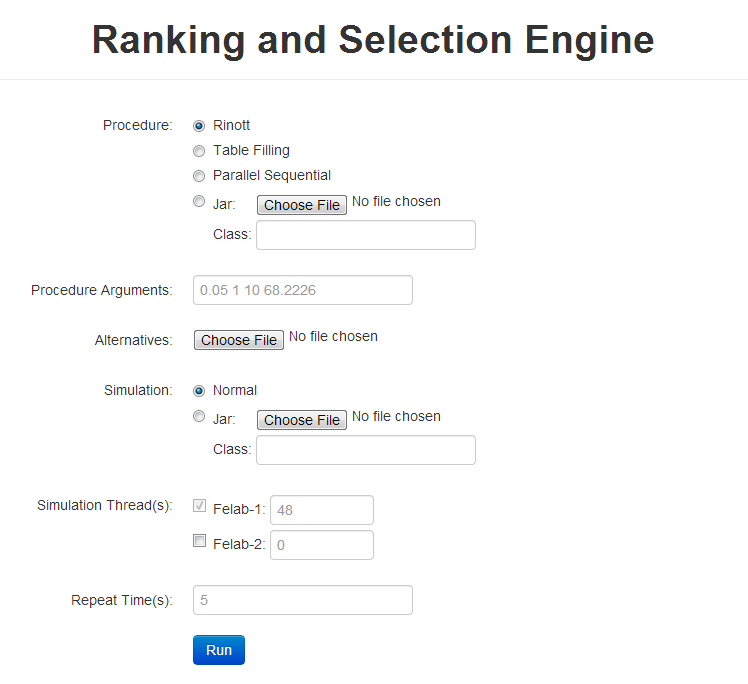
\includegraphics[width=120mm]{rase_web.png}
\caption{Web UI}
\end{figure}

In this way it is much more user friendly than command line. Beginning users could just choose corresponding R\&S procedure and simulation experiments and fill in the parameters intuitively, advanced users may develop his own simulation experiments, and professional users can develop his own procedure with fairly less effort than what he needs to spend without our work. Interested reader may refer to the appendix to get a detailed user guide of this web interface.

As for the second kind of user interface, we will give a detailed introduction in the section discussing extension points later.

\subsubsection{Scale Out to Cluster}

With a limited number of slave threads inside a single machine, it is very still far way from reaching the bottle neck of the single master structure. In other words, we can get more speed up by simply adding slaves threads.

However, the maximum number of slave threads is empirically limited by the total number of hardware cores on that machine. We can definitely add more slave threads, but without enough hardware parallel executing units, namely cores, it is concurrency in fact, rather than real parallel. Adding more software threads than hardware executing units will hardly gain extra speed up, but will demand more scheduling effort from operating system.

Buying powerful machine with more hardware cores is an approach, which is named as scale up. However the price of the machine will grow much faster than linear against computing power, since the more the machine scales up, the higher technology it requires for manufacturing, which makes the cost increasing dramatically.

A common solution is to compose a cluster with several machines where each of them are not that powerful in single. This is called scale out. We do have worked out a previous implementation which scales out to a small cluster. However, that version does not include features like supporting self-customized R\&S procedure and simulation experiment, since it involves a fundamental refactoring of design. Till this thesis, our latest trunk version have fully supported all the features mentioned in this thesis inside single machine range. We will take scaling out to cluster within latest trunk version as a future work.

\subsection{Extension Points for Universality}

Since there has already been so many different combinations of R\&S procedures and simulation experiments to solve selecting the best problem, it is necessary to extract the common components and define reasonable extension points for different components, which follows an import design principle saying that "don't repeat your self". And it will also help a lot when facing a new selecting the best problem since researchers can focus on the part that the new problem differs from others, as long as the specific solution for the different part is developed strictly against the specifications of extension points stated in the rest of this section.

\subsubsection{Specification of Self-customized Procedure}

The implementation of self-customized R\&S procedure should follow the specification, or function signature below. By the way, it's in Java.

\begin{lstlisting}[language=Java]
public int ras(double[] args, double[][] alts,
        SimHelper simHelper);
\end{lstlisting}

Here the first function argument args stands for the parameters needed to carry out the R\&S procedure. For example, in the Rinott's procedure it will contain $\alpha$, $\delta$ and $n_0$. Programmer should arrange these parameters in this array.

The second function argument alts stands for all the alternatives. Noticed that it is an two-dimension array and each alternative is fully represented by an one-dimension array inside. For instance, in the (s, S) inventory problem, an alternative could be fully represented by two parameters $s$ and $S$ inside that one-dimension array. Usually a programmer would like to add an extra $id$ as the first parameter representing the alternative for convenience.

The third function argument simHelper is a self-defined type, or class in Java, which contains all the needed callable programming interfaces, or pre-build-in functions for implementing a self-customized R\&S procedure. These interfaces will be introduced in the next section.

Throughout the design of these extension points, we will try our best not to involve programming language dependent grammar or feature in the hope of reducing user's learning effort, just like the arrays here is plain array of double which is similar to most C-style languages, rather than advanced data structure like ArrayList provided by Java standard library.

\subsubsection{Interfaces for Self-customized Procedure}

Here comes to the part introducing all the programming interfaces provided for implementing R\&S procedures. Firstly let's look at two plain old java objects, or POJOs for shout, which act like the struct in C-programming language. They are the wrappers for simulation input and output, so we name them as SimInput and SimOutput, respectively. We only list the fields here, and will explain the meaning of each field later during the explanation of programming interfaces.

\begin{lstlisting}[language=Java]
public class SimInput {
	public int syncID;
	public int altID;
	public double[] args;
	public long[] seed;
}
\end{lstlisting}

\begin{lstlisting}[language=Java]
public class SimOutput {
	public int syncID;
	public int altID;
	public double[] result;
}
\end{lstlisting}

As for the programming interfaces for implementing R\&S procedures, they can be divided into two types, one is synchronized interfaces, the other is asynchronized ones.

Generally speaking, programming interfaces, or functions, which appear in pure serial program, are all synchronized. It means that once this function is called, the whole program will "stuck" there until the execution of that function is finished and the result get returned if there exits any.

On the contrary, interfaces appeared in parallel program may be synchronized or asynchronized. Asynchronized means that once the function is called, the function will return almost immediately, without the real execution. The real execution may be delayed to some point later, or may get started already but not yet finished. The caller of this asynchronized function may get informed of the execution result in the future, or may have to make polling request itself to get latest execution status.

The only synchronized interface is provided as:

\begin{lstlisting}[language=Java]
public SimOutput[] sim(int[] altIDs);
\end{lstlisting}

Here the only parameter altIDs is the list of ids of alternatives need to be simulated against, each for once. Duplicated ids appeared in this array is allowed for replicated execution of simulation.

For example, during the implementation of the Rinott's procedure, this interface should be called twice, say, each in one stage. In the first stage the length of this array should be $kn_0$, standing for simulating against all the $k$ alternatives for $n_0$ times. As for in the second stage, the length of this array should be dependent on the result of first stage.

The return value here is an array of SimOutput and each SimOutput stands for the result of one simulation experiment. The order inside this array can be totally different from that in the input altIDs array, which doesn't matter since the altID field is exactly the one from the input altIDs array. The result field will contain the simulation result, using an array to support multiple result values from simulation experiment.

Still in the example of the Rinott's procedure, since this interface is synchronized, it won't return until all the simulation results are ready, which archives an implicit barrier here. In this way, the classic two-staged Rinott's procedure can be fully implemented with this synchronized interface.

To support parallelism in fully sequential procedures, asynchronization is provided through at least two interfaces. One is for sending out simulation requests, the other is for collecting simulation results.

The asynchronized interface for sending out simulation request is provided as:

\begin{lstlisting}[language=Java]
public int asyncSim(int[] altIDs);
\end{lstlisting}

Here the only parameter altIDs is the same meaning as that in the synchronized interface, while it will return immediately with an single int value representing an internal identification for synchronized simulation batch. This value will be used in implementing future procedure.

After calling this interface, the procedure can do what ever it needs to do, or call the asynchronized interface for collecting simulation result, which is provided as:

\begin{lstlisting}[language=Java]
public SimOutput[] takeSimOutputs(int n, boolean block);
\end{lstlisting}

Here the first parameter n is the number of simulation result demanded by caller, the second parameter block is a bool variable with following logic: If this variable is set to true, then this function will not return until n simulation result are ready for taken. Otherwise if this variable  is set to false, then this function will always return immediately no matter the n simulation result is ready. It is possible that only several simulation results are return with the number smaller than n, or no result get returned at all. Caller of this function can judge the situation from the return value.

A typical example of using these asynchronized interfaces is the implementation of the revised fully sequentially procedures. After sending out a certain number of simulation experiment requests, calling takeSimOutputs with $n = 1$ and $block = true$ repeatedly, meaning that the fully sequential procedure could do something after each new sample value. The appending simulation requests are also sent out here, archiving customized sampling rule.

\subsubsection{Specification of Self-customized Simulation}

The implementation of self-customized simulation experiment should follow the function signature specified below:

\begin{lstlisting}[language=Java]
public double[] sim(double[] args, long[] seed);
\end{lstlisting}

Here the first function parameter args is all the parameters needed to identify the alternative against which to run the simulation, namely the configuration of an alternative.

The second function parameter seed is an array of integers needed in generating uniformly distributed random numbers with the MRG32k3a algorithm. The main idea here is to make each simulation independent from each other in the viewpoint of statistic by attaching each simulation experiment a different set of seeds, which is generated in master before sending out the simulation request. What's more, we also need a set of seeds to generate many sets of seeds used by simulation experiments, and the "master seeds" here could be specified by user.

The return value is design as an array to support multiple simulation results.

Generally speaking issues needed consideration in integrating an simulation experiment is much fewer than those in developing a new R\&S procure. The only thing should get attention here is how to use the seeds provided from master reasonably during simulation.

\subsection{Features for Performance}

Till now we have introduced our work in higher level for a efficient and flexible architecture. In this section we will describe two low level designs specifically for better parallel performance. One is to reduce communication cost by buffering the messages with an FIFO queue, the other is to speed up serial comparison by adopting the heap, which is also a common data structure.

\subsubsection{Communication with FIFO Queues}

Direct communication among the master and slaves are quite expensive, in the sense that slaves have to take turns when communicating with master and the master itself needs to guarantee mutual exclusion, which put more burden on the single threaded master. In order to overcome this shortage, we have used an FIFO queue, or a BlockingQueue in Java.

The FIFO queue is is a abstract data structure that all the elements are keep in order and theoretically only two operations are supported. One is enqueue, which appends one element to the end of queue, the other is dequeue, which extract one element at the beginning of the queue. Both of them have $O(1)$ complexity. In parallel environment, the enqueue operation will stuck there if the queue is full, and it's the same for dequeue operation if the queue is empty.

With FIFO queues, the master could just send out simulation parameters to a queue and obtain simulation results from another, thus won't get stuck in most cases. On the hand, slaves can receive simulation parameters from the first queue and put simulation results to the second one. Just like the figure below:

\begin{figure}[ht]
\centering
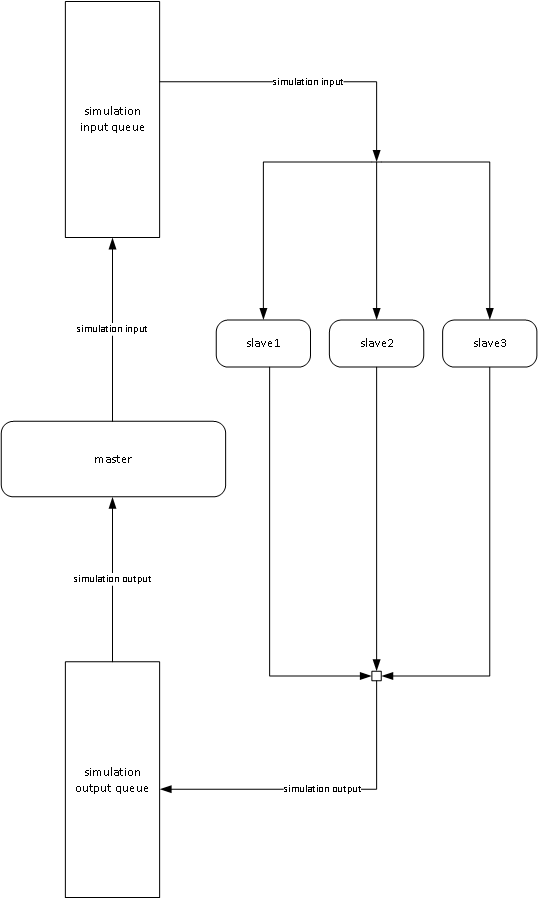
\includegraphics[width=120mm]{master-slave-queue.png}
\caption{master-slave structure with queue}
\end{figure}

In this way, communication cost inside single machine is dramatically reduced for both master and slaves. And if we regard these queues as buffers for parameters and results, it is also possible to make batched communication after scaling to a cluster, which is critical in network communication since with reliable connection-oriented protocol, establishing new connections frequently is much more costly than stable continues transportation.

Except from the performance benefit it has brought in, adopting FIFO queues also helps to decouple the master and slaves, which makes the design more clear.

\section{Numerical Experiment and Analysis}

In this section we will present the numerical results from the latest version of our implementation. We will start from listing the hardware and software environment of our experiment, then present the results when solving the three-stage buffer allocation problem, and finally give an analysis of the result.

\subsection{Hardware Environment}

Our experiment is done on a Dell PowerEdge R815 rack mount server, with four AMD Opteron 6176 CPUs equipped, namely a multi-processor machine. The total memory size is 64GB which is huge enough to support our experiment, and we will need to discuss the limitation from the number of hardware parallel execution units.

\subsubsection{Parallel Execution Units}

Each of the four AMD Opteron 6176 CPUs has 12 cores, thus 48 cores in total. Information from /proc/cpuinfo on operating system has also verified this hardware configuration.

Empirically it is possible to start more than 48 tasks at the same time. Besides, it is also quite proper since using up the computing ability of each machine is a way to reduce IT cost. Engineers in IT industry have even tried to study the most aggressive ratio of software parallel tasks over hardware parallel execution units, which highly depends on detailed scenario but is definitely no less than 1.

In our experiment, in order to guarantee an good parallel computing status among all slave threads, we set the number of slaves to 48 in maximum, which is quite conservative.

\subsection{Software Environment}

Commercial software components like the Windows from Micro Software or Matlab from MathWorks are not suitable for building systems which are going to scale out in the viewpoint of licence cost, so we will build our implementation based on software that is free in charge.

\subsubsection{Operating System}

We have installed CentOS 6.2 as the operating system on our server, which is the most popular community supported and server oriented Linux distributions, and the name CentOS itself is short for "Community Enterprise Operating System".

CentOS is extremely stable since it has $100\%$ binary compatibility with its upstream source Red Hat Enterprise Linux, a ceremonially supported and enterprise server level Linux distribution from Red Hat, which is the leading Linux service provider in the world. 

\subsubsection{Runtime Environment}

We have installed Java Runtime Environment 1.6. We choose Java programming language since it is free compared to Matlab and powerful enough with abundant third-party libraries.

Extra benefit with Java includes but not limited to the natural ability of cross-platform, the robustness in the language itself, e.g..

\subsection{Numerical Result}

The numerical result is taken from solving a specific instance of the three-stage allocation problem with a fairly large scale. We have repeatedly run the experiments with different number of slave threads against this problem and finally have complete correctness and good parallelism archived.

\subsubsection{The Problem Scale}

The feasible region of this instance of three-stage allocation problem is defined as $x_1 + x_2 + x_3 \leqslant 20$, $x_4 + x_5 = 20$, $1 \leqslant x_i \leqslant 20$ and all the $x_i$ are natural number, so there are 21660 feasible solutions in total, in other words the $k = 21660$ here.

In previous time this scale size makes it thought as not suitable for solving by R\&S, and often dealt with through methods like OvS. In our experiment it is solved with an affordable time cost, which will be shown later.

\subsubsection{Correctness}

From the IZ viewpoint introduced before, both the best solutions and the ones which are within $\delta$ difference from the best solutions can be regarded as correct selection.

In this specific problem instance, all the correct selections can be obtained in advance through other methods, which let us to verify the correctness of results obtained from running our own R\&S implementation. The correct results are listed below:

\begin{table}[ht]
\begin{center}
\begin{tabular}{|c|c|}
\hline
Alternative & Comment \\
\hline
(6, 7, 7, 12, 8) & best \\
(7, 7, 6, 8, 12) & best \\
(6, 7, 7, 13, 7) & good \\
(7, 7, 6, 7, 13) & good \\
(6, 7, 7, 11, 9) & good \\
(7, 7, 6, 9, 11) & good \\
\hline
\end{tabular} \\
\caption{Results Obtained in Advance}
\end{center}
\end{table}

Again noticed that the best answers and the good enough answers are all considered as correct selection.

The corresponding log has shown that we archived correct selection every time running our implementation, regardless of different parallel configurations each time. This is also the basic requirement of our work. With the guaranteed correctness, we can focus on the performance data now.

\subsubsection{Performance}

Here we will report the total number of samples generated during R\&S and the total time spent during the whole program. The total number of samples can be regarded as total simulation workload approximately, which should be carried out by all the slaves in parallel. As for the total time cost, that is the most data we're interested in developing this implementation. Below is the detailed results:

\begin{table}[ht]
\begin{center}
\begin{tabular}{|c|c|c|c|c|c|c|}
\hline
Num. of Slaves(n): & 1 & 4 & 8 & 16 & 32 & 48 \\
\hline
Sample Size($\times 10^5$) & 2.426 & 2.434 & 2.442 & 2.442 & 2.433 & 2.436\\
\hline
Elapsed Minutes(t): & 370.5 & 129.4 & 94.4 & 68.3 & 41.7 & 34.2 \\
\hline
\end{tabular} \\
\caption{Performance Data}
\end{center}
\end{table}

The time cost reported in this time is at least affordable for research purpose now. By the way, we also monitored the program with a more professional tool named visualvm, interested reader may refer to the appendix.

\subsection{Performance Analysis}

We can see from the table above that the sample size varies very little from number of slaves, which implies that the simulation work load is almost fixed. According to Amdahl's law, the speed up ratio can be modelled as $\frac{1}{(1 - p) + \frac{p}{n}}$, where $p$ the parallel proportion of the program, $1 - p$ is the remaining serial proportion, and $n$ is the number of processors. Now we would like to estimate $p$ with model below:

$$ t = a \times (1 - p + \frac{p}{n}) + \epsilon $$

Here $a$ is the factor, $\epsilon$ is the noise, and we can get t and n from the result table above. The model can be turned into: 
$$ t = (a - ap) + ap \times \frac{1}{n} + \epsilon $$

With linear regression, we can get $a - ap = 40.4$ and $ap = 332.9$ with $R^2 \geqslant 0.994$, so $p$ is 0.892, which means 89.2\% of simulation work is paralleled.

This parallel ratio fits the R\&S feature that intuitively most workload can get executed in parallel, and also get benefited from all the design decisions and programming techniques with the purpose of reducing the serial workload. It can be considered as a good starting point of scaling out to more execution units, where a cluster rather a single machine will be involved.

\chapter{Comparison Acceleration}

Heap is a widely used data structure in computer science. It is a tree-based data structure, whose node contains a key value for comparing and sorting. For min-heap, the key value of each node is greater than or equal to that of its parent if exists and less than or equal to that of its children also if exists. For max-heap, the situation is just opposite. This is called heap property.

Here we borrowed an example of max-heap from \url{http://en.wikipedia.org/wiki/Heap_(data_structure)}. It can be seen easily that the number in each parent node is greater than or equal to its child nodes if exists.

\begin{figure}[ht]
\centering
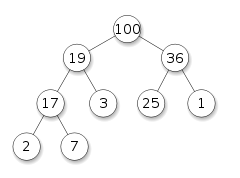
\includegraphics[width=64mm]{heap.png}
\caption{max-heap example borrowed from wikipedia}
\end{figure}

With such heap property, the root node of heap contains the min(max) key value among the whole tree. Operations defined on heap and corresponding time complexity is listed below:

\begin{itemize}
\item insert node with certain key value: $O(\log n)$
\item find node with min(max) key value: $O(1)$
\item update key value of certain node after the node is located: $O(\log n)$
\item remove node with min(max) key value: $O(\log n)$
\end{itemize}

One more thing to mention here is that the complexity of finding node with certain key value should be $O(n)$ in general, since it requires a full scan of the whole data structure. We played a trick here in this specific scenario, where the node of this heap stands for an alternative with statistic information of its sample values. We used an external array, since the ids of alternatives are natural numbers from $0$ to $k - 1$, to track the internal location of corresponding alternative node inside the heap, namely we have implemented our own heap which differs from the one in Java standard library to support $O(1)$ complexity query from alternative id to corresponding statistic information.

After we have customized the heap to support $O(1)$ query in our scenario, now we can discuss our comparing algorithm, digging into the case where we need to select the alternative with minimum mean, since selecting the maximum is quite similar. In this case, alternative i dominates alternative j is equivalent to:

$$ \bar{X}_j(n_j)-\bar{X}_i(n_i) \ge \max\{0,a(\frac{S_i^2}{n_i}+\frac{S_j^2}{n_j}) - b\} $$

From the coding viewpoint, for any updated alternative, which just received an new sample value in fully sequential case, to check whether it dominates other alternatives or be dominated, we need three steps.

Step one is to consider the extreme scenario, although seldom occurs, where $a(\frac{S_i^2}{n_i}+\frac{S_j^2}{n_j}) - b < 0$. To see whether it really happens, just check from the updated alternative and the alternative whose $\frac{S^2}{n}$ is largest among all the alternative except the updated one. If so, one of the two alternatives will be eliminated immediately. For the elimination of the updated alternative, the whole comparing algorithm is done and we can move on directly to next sample value, while for the the elimination of the other one, this step will be repeated. In this way, maintaining a max-heap of alternatives with their $\frac{S^2}{n}$ as sorting key value will save us from looking for the next alternative whose $\frac{S^2}{n}$ is largest among all the survived alternative except the updated one with O(n) time complexity every time repeating this step.

After consideration of extreme scenario, alternative i dominates alternative j only happens when
$$ \bar{X}_j(n_j)-\bar{X}_i(n_i) \ge a(\frac{S_i^2}{n_i}+\frac{S_j^2}{n_j}) - b $$
since for any pair of survived alternatives i and j, $a(\frac{S_i^2}{n_i}+\frac{S_j^2}{n_j}) - b \ge 0$ always holds.

With basic algebra operation, say moving items from one side of equation to the other, the two alternatives can be separated into different sides, e.g.
$$ \bar{X}_j(n_j) - a \times \frac{S_j^2}{n_j} \ge \bar{X}_i(n_i) + a \times \frac{S_i^2}{n_i} - b $$

Now the whole thing comes to light. To see whether the updated alternative dominates any other surviving alternatives, just check from the alternative with largest $\bar{X}(n) - a \times \frac{S^2}{n}$, repeatedly if any elimination happens. This is step two actually and another max-heap of alternatives with $\bar{X}(n) - a \times \frac{S^2}{n}$ as its sorting key value is maintained, for the possibility of repeated elimination.

The third step is even simpler, just checking the survival of the updated alternative against the alternative with smallest $\bar{X}_i(n_i) + a \times \frac{S_i^2}{n_i}$ and no iteration is needed here.

During the whole comparison, time complexity for every possible elimination is $O(\log n)$, under the condition that locating any certain alternative inside a heap costs less than, at most equal to $O(\log n)$. This is satisfied by the customization we have made on standard heap.

What's more, if there's no elimination during the comparison, which occurs frequently in experiments, the time complexity will be reduced to $O(1)$, since no adjustment of any data structure is needed. That's why our comparing algorithm performs much better than $O(\log n)$ in average.

\chapter{Conclusions and Future Work}

In this thesis we have introduced our parallel implementation of both classic Rinott's procedure and two revised fully sequential procedures. Basically it is master-slave structure in higher level and the core components are extracted out while the procedures are implemented as plug-ins, which makes it open for self-customized procedures. Meanwhile, performance is also considered carefully with suitable data structure like FIFO queue and heap adopted, and numerical experiments also showed that the parallel ratio of the whole program is pretty high which guarantees the scalability.

However, there is still much room left for future improvement. The most exciting possibility is to make it the stand benchmark for all the previous and future R\&S procedures by providing this implement as a service in the form of cloud computing. Before that, some critical issues should be considered carefully, like the scalability after a cluster getting involved, the difficulty for a user developing R\&S procedure as plug-in of our implementation, e.g.

Besides, as there exist so many different simulation R\&S procedures, it is necessary to build an uniform platform to compare their performance in parallel computing environment empirically. Although previous work like \cite{ms05ras} has already made an comparative study, they only work on the serial computing environment.

\newpage
\addcontentsline{toc}{chapter}{Appendix}
\appendix

\chapter{Common Parallel Patterns}

A pattern is a tested solution to a certain kind of problem under some conditions. Here we have summarised several common patterns in parallel computing and listed them below.

\section{Embarrassingly Parallel}

Embarrassingly parallel looks more like a problem rather than a pattern. It deals with problems where separating the original problem into smaller ones takes very little or no effort at all. This happens when no communication or dependence exists among separated small problems, for example, if all sub-problems just need to do the same operation and they are independent from each other.

Some problems can be turned into embarrassingly parallel easily. For example, if all sub-problems dependent only on global data structure, then just replicate global data to all sub-problems thus being embarrassingly parallel.

\section{Pipeline}

Pipeline is a classic pattern or architecture. We have already introduced hardware pipelines inside processor cores in section 3.1.2, and here we will introduce software pipeline pattern or architecture, for parallel purpose.

Software pipeline is composed of several threads or processes, which depends on implementation. A continuous data stream flows into the first thread or process as input and pass corresponding output as input to next thread or process. It continues so that every thread or process can do certain action on part of data simultaneously.

The most popular software pipeline should be Unix pipeline. It composes Unix commands into a pipeline with simple $\mid$ signs, which makes Unix shell extremely strong and flexible. It is implemented with multiple processes.

\section{Master-Slave}

Master-Slave pattern or architecture may be the easiest one to implement on distributed environment. In a Master-Slave structure, a master process takes care of the essential serial part of the whole parallel program, while several slaves execute the paralleled workload. Any slave who finishes current workload will inform the master and wait for master's response, like starting a new task. The figure later in this section is a brief illustration of how master-slave pattern works.

\begin{figure}[ht]
\centering
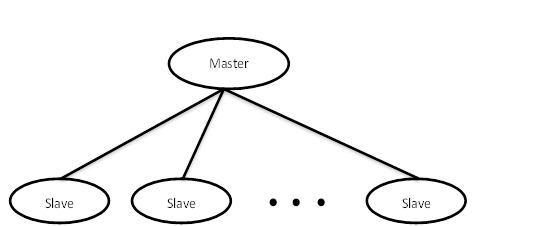
\includegraphics[width=120mm]{master-slave-brief.png}
\caption{A brief illustration of master-slave pattern}
\end{figure}

Since master does serial part and takes extra cost like coordination, it is very easy to become the bottle neck of whole parallel program, although get multi-levelled. We will give a deeper analysis in the next chapter since we adopted this pattern or architecture in our implementation.

Master-Slave pattern is a high-level abstract pattern. There're many specific instances, like fork-join. 

Fork-join maybe the simplest instance of master-slave structure. In this instance the master will start or fork many slaves first, then wait for or join the finish point of all the slaves, with a barrier generally.

Master-Slave structure is so high-level abstract that even the Hadoop map-reduce, which we will introduce in the next section, has a master-slave structured underlay.

\section{Map-Reduce}

This pattern has become hot in recent years due to Google's publication \cite{google-map-reduce} followed by Apache's open source implementation named Hadoop. The key idea is to first split original data set into small pieces and perform the same operation called "map" on these data pieces, turning every data piece into key-value pair format. Then perform the same operation called "reduce" on the intermediate key-value pairs and finally combined them together to get final result.

It is much more than a theoretical pattern because of the Hadoop framework. It has covered many parallel implementation details so that programmer can focus on the business logic part, say, "map" operation and "reduce" operation. The only left difficult point for programmers is how to fit original problem into such two steps.

\section{Parallel Pattern Conclusion}

Parallel patterns listed above are common and intuitive. They take advantage of data decomposition and functional decomposition, but rely heavily on the natural presentation of original problem and fit problem into suitable patterns.

To expose better parallelism, advanced tricks are involved like Fast Fourier Transform to take advantage of specific domains, which are not that common any more.

Besides, patterns are more art than science. It is not necessary to stick strictly to some pattern as long as the problem get solved.

\chapter{User Guide of RASE}

To develop your own simulation code, the following steps are suggested:

1.	Install eclipse (\url{http://www.eclipse.org});

2.	Inside eclipse, File $>$ New $>$ Java Project and follow the wizard;

3.	Import rase-sim-1.0.jar, which can be found \url{http://143.89.20.47/rase/guide/rase-sim-1.0.jar}.

4.	Write your own simulation code, which needs to implement the Sim interface, like the example \url{http://143.89.20.47/rase/guide/NormalSim.java}. This example just returns a normally distributed sample value.

To implement the Sim interface, you only need to implement one method:

\begin{lstlisting}[language=Java]
public double[] sim(double[] args, long[] seed)
\end{lstlisting}

Here args is the arguments that distinguish an alternative, while seed determines the result of this simulation. The output should be an array of double.

5.	Package your project into a jar file. Just right click the project $>$ Export $>$ Java $>$ JAR file, and follow the wizard.

After developing the jar file, please move to \url{http://143.89.20.47/rase/}. If the server is available, you will see a form about ranking and selection configuration, namely the figure in \ref{web-ui}. We will give a detailed description here.

1.	Procedure part:

If you only focus on the simulation part, please just choose build-in procedure and fill in the argument like example.

2.	Alternatives:

You need a plain text file specifying the configuration of each alternative, one line for each alternative. When running simulation for some certain alternative, the corresponding line will be passed as the args to the sim function you have just written. \url{http://143.89.20.47/rase/guide/normal.5.alts} is an example describing five alternatives, related to the simulation example mentioned before.

3.	Simulation

Just choose Jar and upload your jar file, and specifying the class(including package name)

4.	Simulation Threads

Currently e we only support single machine version, which means that you can specify the number of threads on Felab-1. We will support cluster version later.

5.	Repeat Times:

It’s the number of replication.

If you want to develop your own ranking and selection code, the steps are quite similar, except that the jar file that needs to import is \url{http://143.89.20.47/rase/guide/rase-ras-1.0.jar}, and we have these examples, they’re Rinott’s Procedure (\url{http://143.89.20.47/rase/guide/RinottRas.java}), Table Filling Procedure (\url{http://143.89.20.47/rase/guide/TableFillingRas.java}) and Parallel Sequential Procedure (\url{http://143.89.20.47/rase/guide/ParallelSequentialRas.java}).

This time you need to implement Ras interface, which also only contains one function:

\begin{lstlisting}[language=Java]
public int ras(double[] args, double[][] alts,
        SimHelper simHelper)
\end{lstlisting}

Here args is the ones that passed from the webpage, while alts is read in from the file uploaded. To understand the usage of SimHelper, please see the examples above and the corresponding Java doc.

\chapter{Status Monitoring}

We have monitored the execution of our program with visualvm, which is a monitoring tool inside the official Java development kit. Here we put an screenshot when the number of slave is 4.

\begin{figure}[ht]
\centering
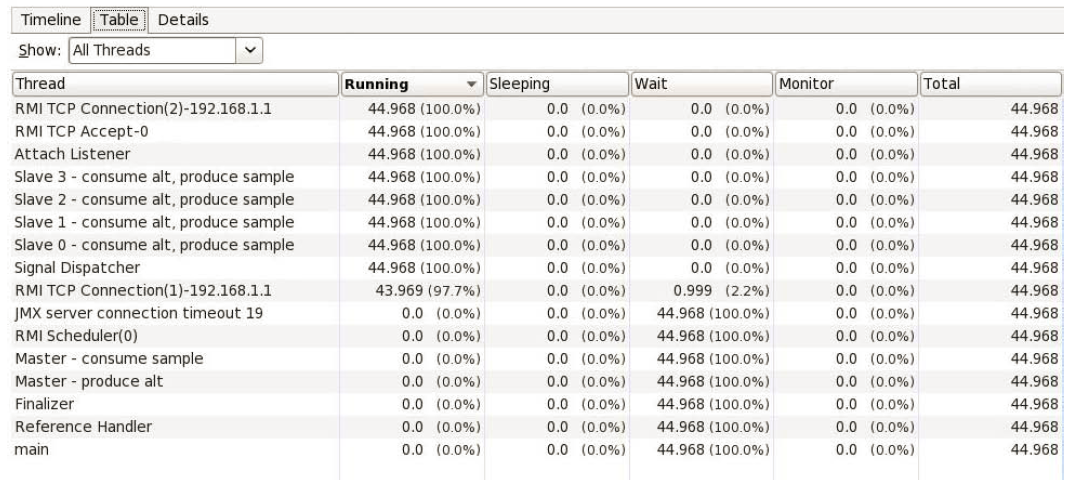
\includegraphics[width=128mm]{monitor.png}
\caption{a monitoring screenshot when the number of slaves is 4}
\end{figure}

It shows that except from the threads that serve for ranking and selection, there're still other threads running for other purposes.

\newpage
%\nocite{*}
%\bibliographystyle{plain}
\bibliographystyle{ieeetr}
\addcontentsline{toc}{chapter}{Bibliography}
%\bibliography{thesis}

\begin{thebibliography}{99}

\bibitem{ras-seq-parallel} J. LUO, L. Jeff HONG, Barry L. Nelson, Y. WU. Fully Sequential Procedures for Large-Scale Ranking-and-Selection Problems in Parallel Computing Environments. Operation Research, 2013.

\bibitem{potwsc11ras} J. LUO, L. Jeff HONG. Large-scale ranking and selection using cloud computing. Proceedings of the 2011 Winter Simulation Conference, 4051–4061.

\bibitem{ras-seq-jeff} L. J Hong. Fully sequential indifference-zone selection procedures with variance-dependent sampling. Naval Research Logistics, 53:464-476, 2006.

\bibitem{ras-recent-advances} Seong-Hee Kim, Barry L. Nelson. Recent Advances in Ranking and Selection. Winter Simulation Conference, 2007.

\bibitem{ehiorams06ras} Kim, S. H. and B. L. Nelson. Elsevier Handbooks in Operations Research and Management Science: Simulation, Chapter 17. Selecting the best system, pp. 501–534. Elsevier.

\bibitem{ms05ras} Jurgen Branke, Stephen E. Chick, Christian Schmidt. Selecting a Selection Procedure. Management Science, 2005.

\bibitem{cistam1978rinott} Rinott, Y. On two-stage selection procedures and related probability-inequalities. Communications in Statistics - Theory and Methods A7, 799–811.

\bibitem{rinott-constant} Wilcox, Rand R. A Table for Rinott's Selection Procedure. Journal of Quality Technology, April 1984, pp. 97-100.

\bibitem{tomacs01kn} Kim, S. H. and B. L. Nelson. A fully sequential procedure for indifference-zone selection in simulation. ACM Transactions on Modeling and Computer Simulation 11, 251.273.

\bibitem{or01nsgs} Nelson, B. L., J. Swann, D. Goldsman, and W. Song. Simple procedures for selecting the best simulated system when the number of alternatives is large. Operations Research 49, 950–963.

\bibitem{potwsc09ovs} Hong, L. J. and B. L. Nelson. A brief introduction to optimization via simulation. Proceedings of the 2009 Winter Simulation Conference, 75–85.

\bibitem{potwsc05ras} Chen, E. J. Using parallel and distributed computing to increase the capability of selection procedures. In Proceedings of the 2005 Winter Simulation Conference, pp. 723–731.

\bibitem{toams1954iz} Bechhofer, R. E. A single-sample multiple decision procedure for ranking means of normal populations with known variances. The Annals of Mathematical Statistics 25, 16–39.

\bibitem{nyjws95iz} Bechhofer, R. E., T. J. Santner, and D. M. Goldsman. Design and Analysis of Experiments for Statistical Selection, Screening, and Multiple Comparisons. New York: John Wiley \& Sons.

\bibitem{google-map-reduce} D. Jeffrey, G. Sanjay. MapReduce: Simplified Data Processing on Large Clusters. Google Inc., 2004.

\bibitem{amdahl} Amdahl, Gene M. Validity of the single processor approach to achieving large scale computing capabilities. Proceedings of the April 18–20, 1967, spring joint computer conference: 483–485.

\bibitem{gustafson} Gustafson, John L. Reevaluating Amdahl's law. Communications of the ACM 31 (5): 532–533.

\bibitem{pca97} Singh, David Culler; J.P. Parallel computer architecture ([Nachdr.] ed.). San Francisco: Morgan Kaufmann Publ.

\bibitem{cotacm90fuji} Fujimoto, R. M. Parallel discrete event simulation. Communications of the ACM 33, 30–53.

\bibitem{scsmasm10fuji} Fujimoto, R. M., A. W. Malik, and A. J. Park (2010). Parallel and distributed simulation in the cloud. SCS Modeling and Simulation Magazine 1.

\bibitem{cissac1985ss} Koenig, L. W., and A. M. Law. A procedure for selecting a subset of size m containing the l best of k independent normal populations, with applications to simulation. Communications in Statistics: Simulation and Computation 1985 14:719–734.

\bibitem{smoms93threestage} Buzacott, J. A., and J. G. Shanthikumar. Stochastic Models of Manufacturing Systems. 1993.

\bibitem{moore} Moore, Gordon E. Cramming more components onto integrated circuits. Electronics Magazine.

\end{thebibliography}

\end{document}
